%% nature.tex — Nature-format submission of the stablecoin basket paper.
%% Format target (Nature, Article): title <=75 chars, summary <=200 words,
%% ~2,500-2,800 words of main text with 4 display items, separate Methods.
%% Numbered references. Build: xelatex/bibtex/xelatex x3 with BIBINPUTS="../;./".
\documentclass[12pt]{article}
\usepackage[margin=1in]{geometry}
\usepackage[T1]{fontenc}
\usepackage[utf8]{inputenc}
\usepackage{lmodern}
\usepackage{amsmath,amssymb,amsthm,mathtools}
\usepackage{graphicx}
\usepackage{booktabs}
\usepackage{float}
\usepackage[section]{placeins}
\usepackage{enumitem}
\usepackage[super,comma,sort&compress]{natbib}
\usepackage[colorlinks=true,linkcolor=black,citecolor=black,urlcolor=black]{hyperref}
\usepackage{setspace}
\usepackage{lineno}
\linenumbers
\onehalfspacing

\newcommand{\Mconf}{\mathcal{M}}
\newcommand{\Mpeg}{\mathcal{M}_{\mathrm{peg}}}
\newcommand{\Bpeg}{\mathcal{B}}
\newcommand{\Wpeg}{\mathcal{W}}
\newcommand{\Sigmait}{\Sigma}
\newcommand{\Covit}{C}
\newcommand{\Deltait}{\Delta}
\newcommand{\Omit}{\Omega}

\title{\Large Correlation rigidity and contagion in\\[1pt]\Large stablecoin baskets}
\newif\ifanon
\ifdefined\ANONBUILD\anontrue\fi
\ifanon
  \author{}
\else
  \author{Hongjun Gou\thanks{Industrial and Commercial Bank of China, Beijing 100140, China. Email: \texttt{gouhongjun\_bs@cq.icbc.com.cn}.}}
\fi
\date{}

\begin{document}
\maketitle

\noindent\textbf{%
Stablecoin baskets now sit underneath a growing share of crypto settlement, and the margins, audits and index products built on them all depend on one quantity: how the coins in a basket move together when one of them breaks its peg. That quantity is never observed directly. On a typical day only a handful of coins deviate from par at all, so the correlation matrices that institutions publish are smoothed across the gaps where data are thin. Here we show that the gaps are not thin data but structural boundaries. Co-movement is constant within each regime defined by a failure channel---collateral backing, price feeds, redemption access, custodianship, bridges, regulation, funding basis and interest margins---and jumps across the boundary between regimes. The jump is supported on the coins that the failing channel touches, it is signed, and no locally smooth estimator can reproduce it. We give a test for the resulting pattern that uses only public price data and apply it to the documented de-peg episodes of the past six years. On the largest custodial failure in the record the pattern appears as predicted, including on a pair of coins that excludes the coin that failed.%
}

\section*{The object being priced}

A stablecoin basket is a portfolio of tokens each of which claims to be worth one dollar. Basket margin at centralised venues, index perpetuals on decentralised ones and proof-of-reserves programmes at regulated issuers all price the same thing: the joint behaviour of the basket when the claim fails for one of its members. What they need is the joint distribution of peg deviations, and in practice what they use is its second moment, the correlation matrix.

That matrix is not observed. On a representative day only three or four coins in a panel of dozens deviate from par at all, and the rest supply a flat line of near-zero returns. A correlation computed on such data is dominated by that flatness, and the matrices that clearinghouses, index providers and regulators publish are consequently smoothed across the gaps where the deviations are missing. The smoothing is usually defended as interpolation: with only a handful of non-trivial observations, some regularisation is unavoidable.

\section*{Why the gaps are structural}

We argue that this defence is misplaced, because the gaps are not sampling artefacts. They are regime boundaries. A stablecoin's peg survives or fails according to structural conditions that change discretely: whether its collateral backs it at par \citep{LyonsViswanath2023}, whether its price feed is still reporting \citep{LiuLiSprenger2023}, whether redemption is open or gated, whether the custodian holding its reserves is solvent \citep{MaZengZhang2023}, whether a bridge has been compromised, whether a regulator has intervened, whether the basis on the funding leg has compressed, and whether a PSM buffer still absorbs the spread. Each of these is a channel through which a basket can be stressed, and each has a threshold.

Within a regime - a region of the parameter space in which no channel has crossed its threshold - the joint co-movement structure of the basket does not change. It is not that it changes slowly; it does not change. Across a threshold it steps. Figure~\ref{fig:wall} shows the geometry for the two channels that admit a continuous representation, collateral backing and price-feed deviation, and locates the remaining six as discrete triggers.

The consequence for correlation modelling is direct. A smooth surface fitted to within-regime data has no way to represent the step, because the step is not in the data it is fitted to: within a regime there is nothing to fit. No amount of additional within-regime data improves the estimate at the boundary, and a smoother that is continuous in the parameters will place at the boundary a value that the true correlation never takes.

\section*{What we posit, and what follows}

We make three assumptions, and we state them as assumptions rather than deriving them, so that a reader can separate what the paper guarantees from what it claims.

The first is that within a regime the co-movement covariance of the basket is constant up to a positive scale. The scale is allowed to move, because the general level of peg-deviation volatility plainly does move; what is fixed is the proportionality structure. We define the covariance as a centred second moment of the peg-deviation vector under the probability law of that regime, which is the object that a correlation estimated from a window of prices actually recovers.

The second is that across a regime boundary the covariance jumps by a signed sum of rank-one terms. Each term is carried by a direction supported on the coins that the crossing channel affects, so the jump has a block structure: the coins a channel touches move together in a way the rest of the basket does not share. The third assumption is that within an episode the support of the jump is a single group of coins, the wall-affected block, fixed by the channel and not by the data.

Everything downstream of these three is proved. The covariance is stated where the crossing law is admissible, because an additive rank-one jump supported on two or more coins necessarily adds a positive amount to its own diagonal, and a correlation matrix cannot absorb a diagonal increment - its diagonal is one on both sides of the boundary by construction. Passing to correlations through the normalisation map removes the obstruction exactly, because that map assigns the unit diagonal rather than computing it. What survives the passage is not the rank-one structure: the normalising map is a nonlinear congruence, and it destroys that. What survives is a signed footprint in three tiers, positive on pairs whose two coins both lie in the block, of opposite sign on pairs with one coin in and one out, and zero on pairs outside the block. And what follows for any smooth estimator is a gap: a locally continuous surface cannot track a function that is constant on regimes and steps between them, so its distance from the true correlation is of the order of the jump and does not shrink as the boundary is approached.

The same reasoning fixes the sign of the block entries. Differentiating the induced correlation jump with respect to the crossing amplitude shows that a block pair rises at the boundary provided its pre-event covariance lies below the harmonic mean of the two variances, a condition that holds automatically when the two coins' variances are equal and that can fail only for a pair that is both strongly correlated and strongly heteroscedastic before the event.

\section*{Testing the block signature}

The three-tier footprint suggests a test that does not require the crossing amplitude, the regime parameters, or any distributional assumption. Classify every pair of coins in an episode by how many of its members lie in the wall-affected block, and ask whether the change in correlation from the pre-event window to the acute window is largest on the block layer. Because a crisis raises co-movement across the whole panel and not only inside the block, the comparison that carries the inference is the block-versus-rest contrast, which differences out a component common to all pairs.

Two details of the inference matter. Pairs share coins and so are not independent, which makes a permutation over pairs anti-conservative; the test we report redraws instead which \emph{coins} form a block of the same size, which asks how unusual the true block is among all the coin sets that could have been so labelled. And because the block is fixed by the channel rather than estimated, the design is a test rather than a fit.

We apply the test to the nine documented de-peg episodes of 2020 to 2025 (Table~\ref{tab:events}), drawn entirely from public price archives. Three of the nine carry a block of more than one coin; the other six involve a single coin and cannot generate a block pair at all.

On the custodial failure of March 2023, in which the reserve custodian of the largest dollar stablecoin failed over a weekend, the block is the three coins exposed through that custodian and through the collateral channel that transmitted the shock: the two largest decentralised stablecoins held the affected token as collateral or as backing. All three layers are ordered as the footprint requires, the block-versus-rest contrast is 0.69, and the coin-level permutation places the true block at the 98.9th percentile of the 816 coin sets of size three that could have been labelled (p = 0.011) (Fig.~\ref{fig:gradient}, Table~\ref{tab:gradient}). The ordering holds across all nine specifications of a window grid that varies the pre-event window between 30 and 90 days and the acute window between three and ten days either side.

The result most exposed to a trivial explanation is the pair formed by the two decentralised coins, which contains neither the token whose custodian failed nor any coin that held reserves at that custodian directly. A victim-only account predicts no jump for this pair. Its members are in the block because the collateral channel touches them, so the test does not establish an effect free of any common exposure; what it establishes is that the effect does not require the coin that actually broke. Its jump, 1.18, is the largest of any pair in the panel.

\section*{Scope of the evidence}

We report the limits as part of the result. Of the two remaining events with a multi-coin block, one is consistent in sign but imprecise, its block-versus-rest contrast positive in eight of nine window specifications, and the other shows no block signal under the canonical window and turns positive only under a 30-day pre-event window. The test therefore finds a clear effect on one episode, a consistent but imprecise sign on a second, and nothing on a third. We do not pool them into a claim about de-peg episodes in general.

Two further conditions bound what the exercise establishes. The block-versus-rest contrast removes a crisis-wide component common to all pairs only if that component is additive and does not differ systematically by layer; we adopt that as an identifying condition rather than as a consequence of the theory, and we report the level of the outside layer so that a reader can see how much of the raw co-movement the subtraction absorbs. And the wall assignment in the historical record draws on post-mortem accounts. In live use the channel is identified by the failure event itself, which is observable as it happens; the instrument described here is therefore a monitor of a channel's incidence, not a forecast of its onset.

\section*{What a supervisor can do with it}

The practical content of the result is narrow and, we think, useful. A supervisor holding only public price data can compute, for any episode, how much more the co-movement of the coins a channel touches has risen than that of the rest of the basket. That statistic requires neither proprietary data nor issuer disclosure, neither of which is available in this market: stablecoin issuers do not publish liquid equity prices and do not disclose bilateral exposures, which is why equity-based systemic-risk measures have found little traction here.

Two uses follow. The first is diagnostic: a supervisor observing a custodial or collateral failure can tell within days whether the basket is transmitting through the channel or merely co-moving with the market, because the two produce different footprints across pair layers. The second is in calibration: a margin or haircut rule that prices the joint tail on a smooth correlation surface will understate it at exactly the moments the surface is asked to carry weight. The size of that understatement is not identified by anything in this paper - the scale of the crossing is left free - but its sign and its support are, and for a rule that needs to know which coins to haircut together rather than by how much, that is the binding input.

The wider point is that stablecoin basket risk is not a smooth function of market conditions but a staircase. Between boundaries nothing happens; at a boundary the structure changes and does not change back until another boundary is crossed. A risk framework that prices the slope is pricing something that, on this evidence, is not there.


\begin{figure}[!ht]
\centering
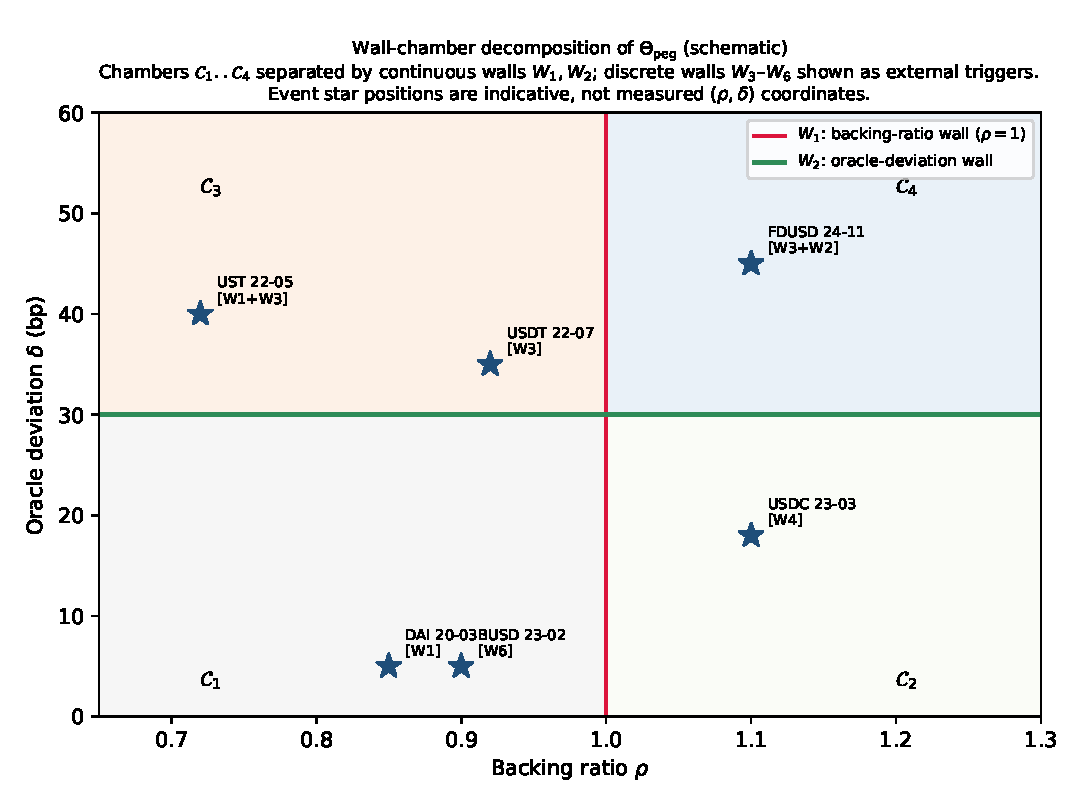
\includegraphics[width=0.62\textwidth]{../figs/fig1_wall_chamber}
\caption{\textbf{Regime boundaries in the peg-preserving parameter plane.} The two channels that admit a continuous representation, collateral backing and price-feed deviation, carve the peg-preserving parameter space into four smooth chambers. The remaining six channels---redemption gating, custodianship, bridges, regulation, funding basis and interest margins---are discrete triggers and are annotated as events rather than drawn as curves. Co-movement is constant inside a chamber and steps across its boundary.}
\label{fig:wall}
\end{figure}

\begin{figure}[!ht]
\centering
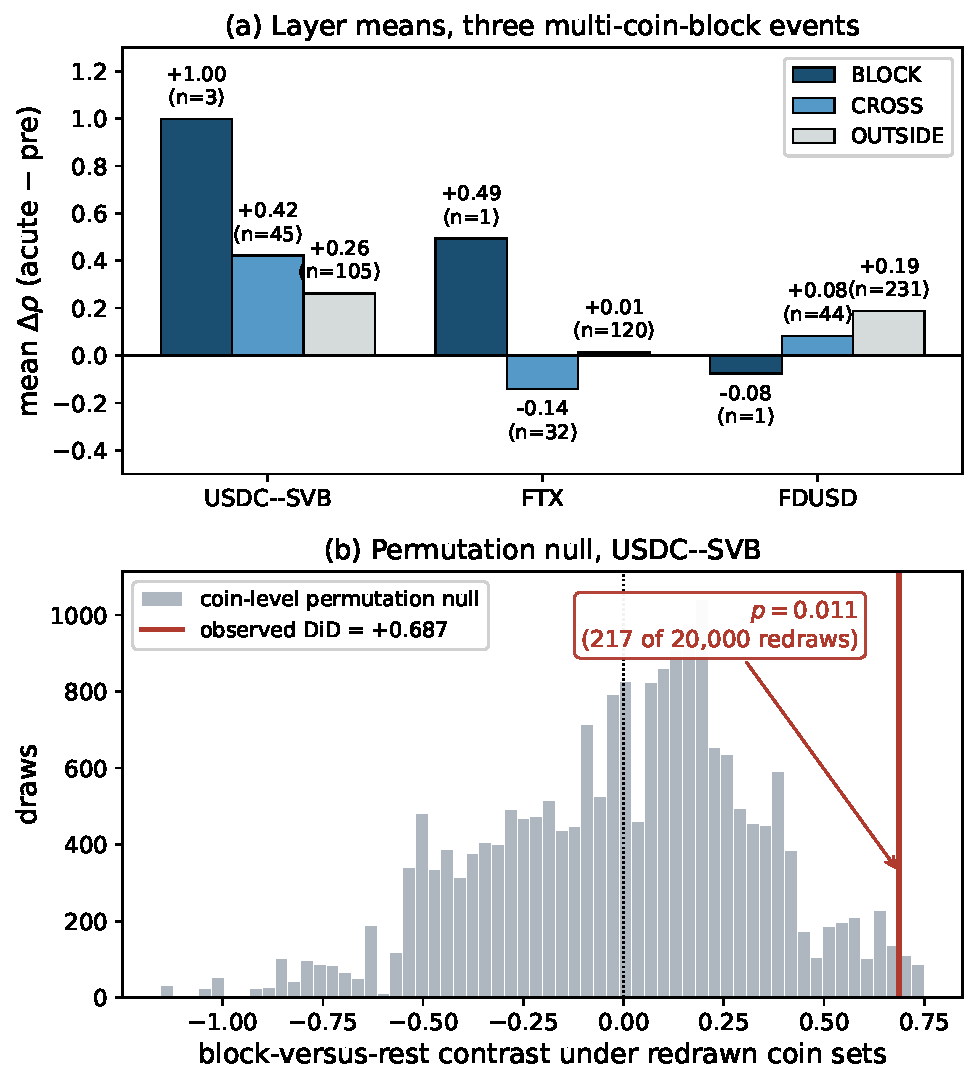
\includegraphics[width=0.9\textwidth]{../figs/fig2_gradient}
\caption{\textbf{The block signature and its permutation null.} \textbf{a}, Change in peg-deviation correlation $\Delta\rho$ from the pre-event window to the acute window, by pair layer, for the three episodes carrying a multi-coin block. Pair counts in parentheses. The predicted ordering holds on the primary episode and on the second; on the third the block layer sits below both others. \textbf{b}, Coin-level permutation null for the primary episode: block labels are redrawn over sets of three coins and the block-versus-rest contrast recomputed for each of 20{,}000 draws. The observed contrast sits in the upper tail.}
\label{fig:gradient}
\end{figure}

\begin{table}[!ht]
\centering
\caption{\textbf{Nine documented de-peg episodes, 2020--2025.} Wall types as in Methods; assignment follows the primary structural failure in the regulator and post-mortem literature. Only three episodes deliver a block of more than one coin, and the pair-level test is defined on exactly those three.}
\label{tab:events}
\small
\begin{tabular}{@{}llll@{}}
\toprule
Episode & Date & Channel(s) crossed & Block \\
\midrule
DAI Black Thursday        & 12--13 Mar 2020 & backing collapse                          & single \\
UST/LUNA collapse         & 09--12 May 2022 & backing $+$ gate                          & single \\
USDT stress episode       & 12--13 Jul 2022 & queue-depth spike                         & single \\
FTX contagion             & 08--14 Nov 2022 & CEX solvency                              & \textbf{multi} \\
BUSD wind-down            & 13 Feb 2023     & regulatory                                & single \\
USDC--SVB weekend         & 10--13 Mar 2023 & custody $+$ backing $+$ gate              & \textbf{multi} \\
FDUSD 2024 event          & 08 Nov 2024     & gate $+$ oracle                           & \textbf{multi} \\
USDe funding-stress       & 02 May 2024     & basis compression                         & single \\
GHO structural sub-peg    & 18 Dec 2024     & interest-rate / PSM                       & single \\
\bottomrule
\end{tabular}
\end{table}

\begin{table}[!ht]
\centering
\caption{\textbf{Pair-level gradient on the three episodes with a multi-coin block.} Entries are layer means of $\Delta\rho$ with pair counts in parentheses; $\widehat{\mathrm{DiD}}$ is the block-versus-rest contrast. $p_{\mathrm{coin}}$ is the coin-level permutation (the operative test), $p_{\mathrm{pair}}$ the pair-level permutation reported for comparison; both one-sided against the no-block null.}
\label{tab:gradient}
\begin{tabular}{@{}lrrrrrr@{}}
\toprule
& BLOCK & CROSS & OUTSIDE & $\widehat{\mathrm{DiD}}$ & $p_{\mathrm{coin}}$ & $p_{\mathrm{pair}}$ \\
\midrule
USDC--SVB & $0.9970$ (3) & $0.4219$ (45) & $0.2619$ (105) & $0.6871$ & $0.0109$ & $0.0025$ \\
FTX       & $0.4937$ (1) & $-0.1404$ (32) & $0.0130$ (120) & $0.5130$ & $0.1553$ & $0.1581$ \\
FDUSD     & $-0.0762$ (1) & $0.0838$ (44) & $0.1867$ (231) & $-0.2464$ & $0.7671$ & $0.7593$ \\
\bottomrule
\end{tabular}
\end{table}

\section*{Methods}

\subsection*{Configuration space and peg preservation}
At a point in time a stablecoin is a tuple $s_i=(C_i,O_i,R_i)$: a collateral composition $C_i$ in the $(K-1)$-simplex over $K$ reserve asset classes, an oracle price vector $O_i\in[0.5,1.5]^J$ with consensus value $\bar O_i=\phi_i(O_i)$, and a redemption gate state $R_i\in\{\text{open},\text{gated},\text{halted}\}$. The signed peg deviation is $\delta_i:=\bar O_i-1$; the backing ratio $\rho_i$ is derived from the collateral and the issuer's outstanding supply and is not an independent coordinate. A state is peg-preserving at tolerance $\varepsilon$ if $|\delta_i|\le\varepsilon$ and the redemption arbitrage cycle is executable with round-trip profitability bounded by $\varepsilon$; the default $\varepsilon=50$ basis points follows \citep{LyonsViswanath2023}. The threshold enters only the definition of peg preservation and is not used as a cut-off anywhere in the estimation.

The configuration space is $\mathcal{M}=\{(s_1,\dots,s_N):\text{joint feasibility}\}$, where joint feasibility comprises backing balance, oracle consistency and redemption clearing; the peg-preserving locus $\mathcal{M}_{\mathrm{peg}}\subset\mathcal{M}$ is the subset on which every coin is peg-preserving. We assume both are non-empty on the parameter range considered. Peg preservation is a constraint cutting a locus out of the ambient space, not a restriction on what the ambient space may contain: de-pegging configurations remain points of $\mathcal{M}$, and the chambers and walls stratify that ambient space.

\subsection*{The three assumptions}
Write $\Theta_{\mathrm{peg}}$ for the parameter range, with coordinates comprising the structural parameters (issuance rule, collateral haircut, oracle bandwidth) together with the state functionals $\rho_i(\theta)$ and $\delta_i(\theta)$ through which those parameters act, so that a condition such as $\rho_i=1$ is read as the level set $\{\theta:\rho_i(\theta)=1\}$ and defines a wall. The wall set is $\mathcal{W}=\bigcup_{k=1}^{8}W_k$; a chamber is a connected component of $\Theta_{\mathrm{peg}}\setminus\mathcal{W}$. Four walls are equalities between a continuous parameter and a threshold (backing ratio, oracle deviation, funding basis, interest spread) and are codimension-one hypersurfaces; the other four are discrete transitions (redemption gate, custody, bridge, regulation). All eight are retained in one list because the crossing each induces has the same rank-one form, but only the first group can be drawn as boundaries in a continuous parameter plane.

For a chamber and a parameter $\theta$ in it, let $\mu_\theta$ be the probability law of $\delta$ while the system sits in that chamber. The law is a primitive of the framework: no dynamics is written down, and the only properties used are that $\mu_\theta$ is a probability measure with finite second moments. The co-movement covariance is the centred second moment
\[
C_{ij}(\theta):=\operatorname{Cov}_{\mu_\theta}(\delta_i,\delta_j),\qquad
C(\theta):=\mathbb{E}_{\mu_\theta}\bigl[(\delta-\bar\delta)(\delta-\bar\delta)^\top\bigr],
\]
which is symmetric and positive semidefinite by construction. The centring is not cosmetic: a coin that trades persistently below par has $\bar\delta_i\ne0$, and an uncentred second moment would not be recovered by any correlation estimate computed on its price series. The normalised image is $\Sigma_{ij}=C_{ij}/\sqrt{C_{ii}C_{jj}}$ on the open set where $C_{ii}>0$, with $\Sigma_{ii}:=1$.

\textbf{(H1) Within-chamber rigidity.} For any two parameter values in the same chamber there is a scalar $\lambda>0$ with $C(\theta)=\lambda C(\theta')$. The scale factor allows the overall level of volatility to drift within a regime while the shape of the co-movement structure is fixed.

\textbf{(H2) Rank-one wall crossing.} Across a wall $W$ separating two adjacent chambers,
\[
C^{+}-C^{-}=\sigma_W\sum_{\gamma\in\Gamma_W}\Omega(\gamma)\,v_\gamma v_\gamma^\top ,
\]
with $\Gamma_W$ a finite set of channels active at $W$, $\Omega(\gamma)\in\mathbb{R}$ signed weights, $v_\gamma$ directions supported on the coins channel $\gamma$ affects, and $\sigma_W>0$ a positive scale. The form is that of the Kontsevich--Soibelman wall-crossing formula \citep{KontsevichSoibelman2008}, which takes a product over the charges whose central charges change sign across a wall and, where it applies, yields a signed sum of rank-one terms on the coins those charges carry. We take that form as the primitive. Two features of the original are not transported: $\Omega$ is not claimed to be an integer, since only the product $\sigma_W\Omega$ is ever identified and integrality would carry no empirical content; and no sign restriction is placed on $\Omega$, so the right-hand side is a general symmetric matrix. The crossing law therefore fixes the support of the jump but not its direction.

\textbf{(H3) Block support.} For each wall crossed by an episode with a multi-coin channel, the directions $\{v_\gamma\}$ span the indicator directions of a single group of coins $B_W$, the wall-affected block; coins outside $B_W$ carry zero weight. $B_W$ is fixed by the channel's structural definition and never by the observed correlation outcomes.

\subsection*{Consequences}
Because $\Sigma_{ii}=1$ on both sides of a wall, the induced correlation jump $\Delta_R:=\Sigma^{+}-\Sigma^{-}$ has zero diagonal identically; no clipping or post-hoc renormalisation is involved. For a single channel with $\Omega=1$ and $v=e_i+e_j$, writing $a:=\sigma_W$, $p:=C^{-}_{ij}$, $X:=C^{-}_{ii}$ and $Y:=C^{-}_{jj}$, the block entry moves by
\[
\Delta_{R,ij}=\frac{p+a}{\sqrt{(X+a)(Y+a)}}-\frac{p}{\sqrt{XY}},
\]
whose derivative at $a=0$ is $(XY)^{-1/2}\,[1-p(X+Y)/(2XY)]$. The block entry therefore rises near the wall precisely when $p<2XY/(X+Y)$, the harmonic mean of the two variances. By the arithmetic--geometric mean inequality that mean is at most $\sqrt{XY}$, with equality exactly when $X=Y$, and $|p|\le\sqrt{XY}$ because $C$ is positive semidefinite; so the condition holds for every admissible $p$ when the variances are equal, and can fail only for a pair that is both strongly correlated and strongly heteroscedastic. The leading coefficient is not $a/\sqrt{XY}$ in general.

A pair with one coin inside the block and one outside behaves differently in sign: because only the inside coin's diagonal moves, $\Delta_{R,ik}=-aC^{-}_{ik}/(2(X)^{3/2}\sqrt{C^{-}_{kk}})+O(a^2)$, which is opposite-signed to $C^{-}_{ik}$ and vanishes exactly when $C^{-}_{ik}=0$. Its size relative to the block entry is of order $|C^{-}_{ik}|/(2C^{-}_{ii})$, small when the pre-event cross-covariance is small relative to the block coin's variance but not bounded away from the block term in general.

Under the midpoint calibration $\Sigma_G(\theta_W)=\tfrac12(\Sigma^{+}+\Sigma^{-})$ at each wall, a Gaussian copula surface $\Sigma_G$ satisfies $\Sigma(\theta^{\epsilon}_{\pm})-\Sigma_G(\theta^{\epsilon}_{\pm})=\pm\tfrac12\Delta_R+O(\epsilon)$ as the wall is approached. The magnitude is a consequence of the midpoint calibration rather than of the Gaussian family; what extends to any smooth surface needs only local continuity - a smooth surface cannot track a function that is constant on chambers and steps between them, so its distance from $\Sigma$ is of the order of the jump and does not vanish.

\subsection*{Panel and windows}
The panel is 28 stablecoins with daily coverage dense enough to enter the panel, drawn from the DeFiLlama public archive over 2020--2025 and cross-checked against Chainlink oracle feeds and CoinGecko quotations; no proprietary or issuer-internal data is used. The pre-event window is the 60 calendar days preceding the event, trimmed to observations with non-missing prices (typically 46 trading days), and ends before the acute window begins; the acute window is the eleven calendar days centred on the event. Because the acute window is centred it contains days on both sides of the crossing, which pulls $\rho^{+}$ toward $\rho^{-}$ and biases $\Delta\rho$ toward zero: the test is conservative in this respect. No pre-window observation enters the definition of $B_W$.

For each event and each pair with at least five usable observations in each window, $\Delta\rho_{ij}:=\rho^{+}_{ij}-\rho^{-}_{ij}$, with $\rho$ the Pearson correlation of daily peg deviations. This is the empirical counterpart of $\Delta_{R,ij}$: the pre-window estimates the pre-crossing chamber value, the acute window the post-crossing value. The identification of a pre-event window with a chamber requires the window to be long enough for the peg-deviation law to settle inside the regime and short enough to precede the event; the first is examinable through the window grid, the second we take as given.

\subsection*{Test and inference}
Pairs are classified BLOCK (both coins in $B_W$), CROSS (exactly one) and OUTSIDE (neither). The tested criterion is that the BLOCK layer mean exceeds both others. The comparison between CROSS and OUTSIDE is reported as an empirical quantity and is not used as a test: the pure crossing law places CROSS below OUTSIDE, since the cross-pair image is opposite-signed, but the observed level of every layer is contaminated by crisis-wide co-movement in proportions this design cannot separate.

A crisis raises co-movement across the whole panel, so the substantive statistic is the block-versus-rest contrast $\widehat{\mathrm{DiD}}=\overline{\Delta\rho}_{\mathrm{BLOCK}}-\overline{\Delta\rho}_{\mathrm{BLOCK}^{c}}$. This is valid only under an identifying condition, which we state explicitly: Assumption (H3) implies that pairs outside the block carry no crossing contribution, so the theory predicts a zero OUTSIDE layer, whereas the observed OUTSIDE means are not zero. A component the theory does not model is therefore present, and $\widehat{\mathrm{DiD}}$ identifies the block effect only if that component is additive and does not differ systematically across layers. We adopt that as a condition, not as a consequence.

Primary inference is a coin-level permutation: the block label is redrawn over sets of coins of the same size as $B_W$ and $\widehat{\mathrm{DiD}}$ recomputed, with 20{,}000 draws, which asks how unusual the true block is among the $\binom{n}{|B_W|}$ coin sets that could have been so labelled. Pair-level permutation, which treats pairs as exchangeable, is reported alongside as the anti-conservative comparison. A coin-level bootstrap interval is also reported; it is conditional on the block assignment, so it measures sampling variability of coins under that assignment rather than the distinctiveness of the block.

\subsection*{Window grid and robustness}
The canonical specification is a 60-day pre-window with a $\pm5$-day acute window, fixed by the panel-construction script before the test was designed. A $3\times3$ grid crosses pre-windows of 30, 60 and 90 days with acute half-widths of 3, 5 and 10 days. The script that produces the grid re-derives the canonical row exactly, which is the check that the grid is comparable across specifications.

\subsection*{The amplitude}
The scale $\sigma_W$ is left free. Because the normalising map is a nonlinear congruence it destroys the rank-one form of the jump, so what survives into correlation space is sign structure and support rather than scale; a test built on those is invariant to $\sigma_W$ at leading order in $a$, which is the order at which the criteria are stated. Fixing $\sigma_W$ would matter only for a test of magnitude, which requires more multi-coin-block events than the record contains.

\subsection*{Data and code availability}
The panel is assembled from public archives (DeFiLlama, FRED, Yahoo Finance, Etherscan) with source URLs, retrieval timestamps, sizes and SHA-256 checksums recorded for every raw file. The reproducibility bundle contains the LaTeX source, all figure-generation and audit scripts, the raw data archive and a checksummed manifest, and the pipeline completes in under three minutes. Code is available at https://github.com/dyzchina/crypto4.


\bibliographystyle{naturemag}
\bibliography{../refs}

\ifanon\else
\section*{Acknowledgements}
The author thanks colleagues at the Industrial and Commercial Bank of China for comments on an earlier draft, and acknowledges the maintainers of the public data archives used here.

\section*{Author contributions}
H.G. designed the study, performed the analysis and wrote the manuscript.
\fi

\section*{Competing interests}
The author declares no competing interests.

\end{document}
